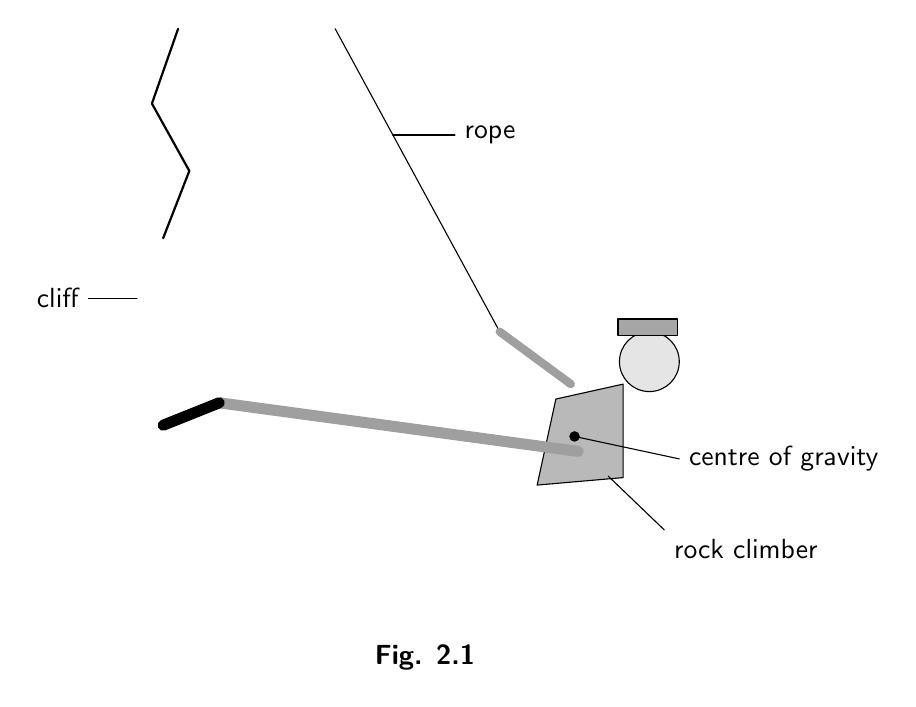
\begin{tikzpicture}[scale=0.95, font=\sffamily, line cap=round, line join=round]
  % cliff face, hatched on the rock side
  \surface{(0,0)}{(0,4.8)}{1}
  \draw[thick] (0,4.8)--(0.35,5.7)--(-0.15,6.6)--(0.2,7.6);
  % rope from the top of the cliff to the climber's hands
  \draw (2.3,7.6)--(4.5,3.55);
  \draw[line width=3pt, gray!75] (4.5,3.55)--(5.45,2.85);
  % body, head, helmet
  \draw[fill=gray!55] (5.0,1.5)--(6.15,1.6)--(6.15,2.85)--(5.25,2.65)--cycle;
  \draw[fill=gray!20] (6.5,3.15) circle (0.4);
  \draw[fill=gray!70] (6.08,3.5) rectangle ++(0.8,0.22);
  % leg pushing against the cliff
  \draw[line width=4pt, gray!75] (5.55,1.95)--(0.75,2.6);
  \draw[line width=4pt] (0.75,2.6)--(0,2.3);
  % centre of gravity
  \fill (5.5,2.15) circle (2pt);
  % labels
  \draw (-0.35,4.0)--(-1.0,4.0) node[left] {cliff};
  \draw (3.07,6.18)--(3.9,6.18) node[right] {rope};
  \draw (5.95,1.62)--(6.7,0.9) node[below right] {rock climber};
  \draw (5.5,2.15)--(6.9,1.85) node[right] {centre of gravity};
  \node[font=\sffamily\bfseries] at (3.5,-0.8) {Fig. 2.1};
\end{tikzpicture}
